\section{Systembeskrivning}

Projektgruppen definierade en tydlig design av applikationen innan implementationen påbörjades. Detta var för att försäkra sig om att applikationen skulle bli av hög kvalitet och eventuella designproblem skulle hittas tidigt i projektet.

\subsection{Systemanatomi}
\label{beskrivning-systemanatomi}
Under iteration ett producerade projektgruppen en systemanatomi av applikationen som skulle utvecklas. Denna producerades utifrån de use-cases och krav kunden hade tillhandahållit. I figur \ref{fig:systemanatomi_graf} visas systemanatomin för hela systemet och i \ref{fig:systemanatomi_spel} visas den för själva spelet.

\begin{figure}[H]
    \centering
    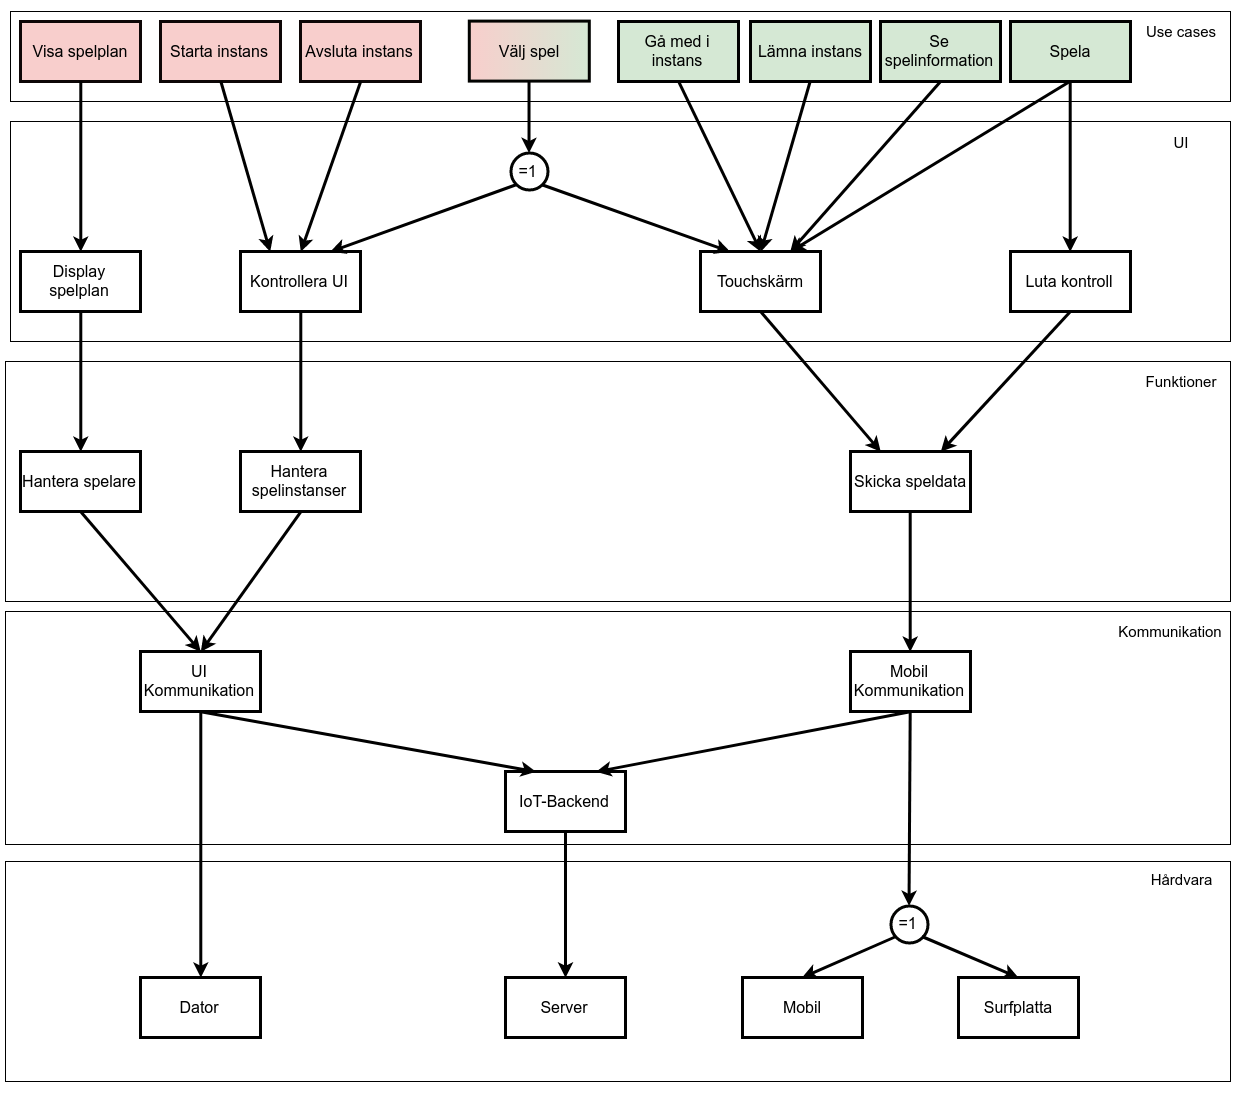
\includegraphics[scale=0.3]{systemanatomi_graf}
    \caption{Överblick av systemanatomin}
    \label{fig:systemanatomi_graf}
\end{figure}

\begin{figure}[H]
    \centering
    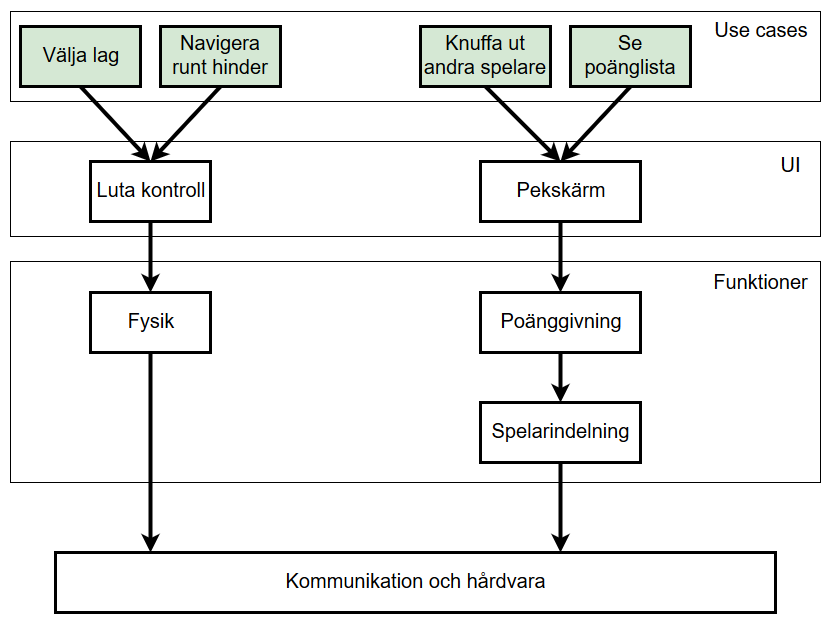
\includegraphics[scale=0.3]{systemanatomi_spel}
    \caption{Överblick av systemanatomin för spelet}
    \label{fig:systemanatomi_spel}
\end{figure}


\pagebreak

\subsection{Moduler}
\label{moduler}
Projektgruppen använde sig av den generella strukturen av systemet, kundens krav och systemanatomin för att skapa en mer detaljerad arkitektur. I figur \ref{fig:konceptarkitektur} kan man se den övergripande strukturen av modulerna som finns i applikationen.

\begin{figure}[h]
    \centering
    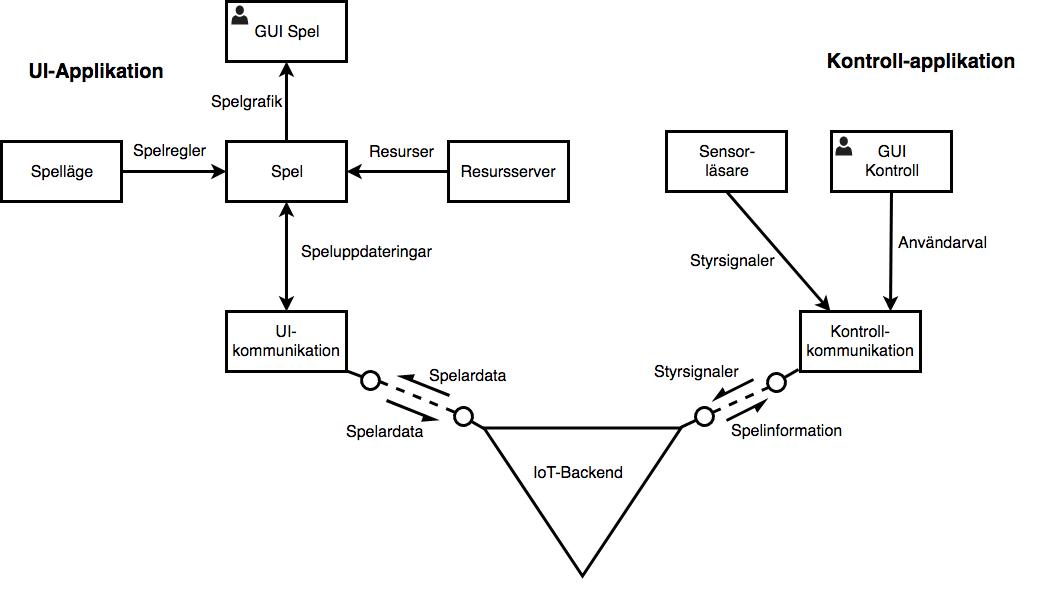
\includegraphics[scale=0.3]{konceptarkitektur}
    \caption{Överblick av systemets moduler}
    \label{fig:konceptarkitektur}
\end{figure}

\pagebreak


\subsubsection*{Ansvarsområden}
Varje modul i systemet har ett eget ansvarsområde. Nedan följer en förtydling på vad varje modul ansvarar för.

\begin{labeling}{\small{\textbf{Kontrollkommunikation}}}
    \item [\small{\textbf{GUI Spel}}]
        \begin{itemize}
            \item Visa upp spelplanen
            \item Visa upp menyer
            \item Starta spel med specifika inställningar
            \newline
        \end{itemize}

    \item [\small{\textbf{Spelläge}}]
        \begin{itemize}
            \item Sätta upp regler för spelet
            \item Avgöra vilka resurser spelet ska innehålla
            \item Avgöra vad som ska ske vid olika tillfällen i spelet
            \newline
        \end{itemize}

    \item [\small{\textbf{Spel}}]
        \begin{itemize}
            \item Hålla koll på de olika spelarna
            \item Tillhandahålla grundläggande spelmekanik
            \newline
        \end{itemize}

    \item [\small{\textbf{Resursserver}}]
        \begin{itemize}
            \item Lagra vilka resurser som finns
            \item Ladda in resurser
            \newline
        \end{itemize}

    \item [\small{\textbf{UI-kommunikation}}]
        \begin{itemize}
            \item Upprätta uppkoppling mot server
            \item Förpacka data för kommunikation
            \newline
        \end{itemize}

    \item [\small{\textbf{Sensorläsare}}]
        \begin{itemize}
            \item Läsa av data från sensor
            \item Abstrahera sensordata till standardiserad form
            \item Konfigurera sensor
            \newline
        \end{itemize}

    \item [\small{\textbf{GUI-kontroll}}]
        \begin{itemize}
            \item Visa menyer för att gå med i spelinstans
            \item Visa spelinformation om det pågående spelet
            \item Tillhandahålla knappar på skärmen
            \newline
        \end{itemize}

    \item [\small{\textbf{Kontrollkommunikation}}]
        \begin{itemize}
            \item Upprätta uppkoppling mot server
            \item Förpacka data för kommunikation
            \newline
        \end{itemize}

    \item [\small{\textbf{IoT-Backend}}]
        \begin{itemize}
            \item Dirigera data mellan olika Kontroll-applikationer och olika instanser av UI-applikationen
            \item Verifiera koder för att gå med i specifika spelinstanser
            \newline
        \end{itemize}
\end{labeling}
